\documentclass[11 pt,a4paper,english]{article}
\usepackage[margin=2.5cm]{geometry} 
\usepackage[T1]{fontenc}     % belső kódrendszer beállítása
\usepackage[utf8]{inputenc}  % input kódolós
\usepackage[english]{babel}   % nyelv

\usepackage[acronym]{glossaries}
\makeglossaries

\usepackage{graphicx} % Képek miatt

\usepackage{adjustbox} % Táblázatokra

 % in the document preamble
\usepackage[stable]{footmisc}

\usepackage{multicol}
\usepackage{wrapfig}
\usepackage{float}

% Keywords command
\providecommand{\keywords}[1] {\small\textbf{Categories and Subject Descriptors:} #1}

\newglossaryentry{NLP}{ type       =\acronymtype,
						name       ={NLP},
						description={Natural Language Processing},
						first      ={Natural Language Processing (NLP)\glsadd{nlpg}},
						see=[Glossary:]{nlpg}
					}
				
\newglossaryentry{SRS}{ type       =\acronymtype,
						name       ={SRS},
						description={Software Requirement Specifications},
						first      ={Software Requirement Specifications (SRS)\glsadd{srsg}},
						see=[Glossary:]{srsg}
					}
				
\newglossaryentry{SDLC}{type       =\acronymtype,
						name       ={SDLC},
						description={Software Development Life Cycle},
						first      ={Software Development Life Cycle (SDLC)\glsadd{sdlcg}},
						see=[Glossary:]{sdlcg}
					}

\newglossaryentry{POST}{ type       =\acronymtype,
						name       ={POST},
						description={Part-of-Speech Tagging},
						first      ={Part-of-Speech Tagging (POST)\glsadd{postg}},
						see=[Glossary:]{postg}
					}

\newglossaryentry{POS}{ type       =\acronymtype,
						name       ={POS},
						description={Part of Speech},
						first      ={Part of Speech (POS)\glsadd{posg}},
						see=[Glossary:]{posg}
					}
\newglossaryentry{nlpg}{name       ={NLP},
						description=
						{
							Natural language processing (NLP) is a subfield of linguistics, computer science, information engineering, and artificial intelligence concerned with the interactions between computers and human (natural) languages, in particular how to program computers to process and analyze large amounts of natural language data
						}
					   }

\newglossaryentry{srsg}{name       ={SRS},
						description=
						{
							A software requirements specifications (SRS) is a description of a software system to be developed. It is modeled after business requirements specification (CONOPS), also known as a stakeholder requirements specification (StRS). The software requirements specification lays out functional and non-functional requirements, and it may include a set of use cases that describe user interactions that the software must provide to the user for perfect interaction.
							Software requirements specification establishes the basis for an agreement between customers and contractors or suppliers on how the software product should function (in a market-driven project, these roles may be played by the marketing and development divisions). Software requirements specification is a rigorous assessment of requirements before the more specific system design stages, and its goal is to reduce later redesign. It should also provide a realistic basis for estimating product costs, risks, and schedules. Used appropriately, software requirements specifications can help prevent software project failure.
							The software requirements specification document lists sufficient and necessary requirements for the project development. To derive the requirements, the developer needs to have clear and thorough understanding of the products under development. This is achieved through detailed and continuous communications with the project team and customer throughout the software development process.
							The SRS may be one of a contract's deliverable data item descriptions or have other forms of organizationally-mandated content
						}
					   }

\newglossaryentry{sdlcg}{name      ={SDLC},
						 description=
						 {
							The Software Development Life Cycle (SDLC), also referred to as the application development life-cycle, is a process for planning, creating, testing, and deploying an information system. There are usually six stages in this cycle: requirement analysis, design, development and testing, implementation, documentation, and evaluation.
						 }
                        }

\newglossaryentry{postg}{name       ={POST},
						description=
						{
							In corpus linguistics, Part-of-Speech Tagging (POST), also called grammatical tagging or word-category disambiguation, is the process of marking up a word in a text (corpus) as corresponding to a particular part of speech, based on both its definition and its context (i.e. its relationship with adjacent and related words in a phrase, sentence, or paragraph).
							Once performed by hand, POST is now done in the context of computational linguistics, using algorithms which associate discrete terms, as well as hidden parts of speech, in accordance with a set of descriptive tags. POST algorithms fall into two distinctive groups: rule-based and stochastic.
						}
					}
				
\newglossaryentry{posg}{name       ={POS},
						description=
						{
							In traditional grammar, a Part of Speech (POS) is a category of of lexical items that have similar grammatical properties. Words that are assigned to the same POS generally display similar syntactic behavior and they play similar roles within the grammatical structure of sentences.
							Commonly listed English parts of speech are noun, verb, adjective, adverb, pronoun, preposition, conjunction, interjection, and sometimes numeral, article, or determiner. Other Indo-European languages also have essentially all these word classes. One exception to this generalization is that most Slavic languages as well as Latin and Sanskrit do not have articles. Beyond the Indo-European family, such other European languages as Hungarian and Finnish, both of which belong to the Uralic family, completely lack prepositions or have only very few of them; rather, they have postpositions.
						}
}

\newglossaryentry{aspiceg}{name       ={ASPICE},
	description=
	{
		Automotive \gls{SPICE} (ASPICE) is a standard made by german car makers. It provides rough guidelines to improve your software development processes and to assess suppliers. This means that practically the whole european automotive industry must follow ASPICE and if you want to know how software development works there it provides a good broad overview.
		Automative \gls{SPICE} is derived from the generic \gls{SPICE} (ISO/IEC 15504) standard. While there are other instances, ASPICE seems to be the only one which got any traction. You can find a lot of ASPICE material on the internet unrestricted by paywalls.
		It builds on the V-Model which means for every process from requirements to source code there is a corresponding test.
	}
}

\newglossaryentry{spiceg}{name       ={SPICE},
						  description=
						  {
							ISO/IEC 15504 Information technology – Process assessment, also termed Software Process Improvement and Capability Determination (SPICE), is a set of technical standards documents for the computer software development process and related business management functions. It is one of the joint International Organization for Standardization (ISO) and International Electrotechnical Commission (IEC) standards, which was developed by the ISO and IEC joint subcommittee, ISO/IEC JTC 1/SC 7.
							ISO/IEC 15504 was initially derived from process lifecycle standard ISO/IEC 12207 and from maturity models like Bootstrap, Trillium and the Capability Maturity Model (CMM).
							ISO/IEC 15504 has been revised by: ISO/IEC 33001:2015 Information technology – Process assessment – Concepts and terminology as of March, 2015 and is no longer available at ISO.
						}
					}
\newglossaryentry{asmg}{name       ={asm},
	description=
	{
		In computer programming, assembly language (or assembler language), often abbreviated asm, is any low-level programming language in which there is a very strong correspondence between the instructions in the language and the architecture's machine code instructions. Because assembly depends on the machine code instructions, every assembler has its own assembly language which is designed for exactly one specific computer architecture. Assembly language may also be called symbolic machine code.
	}
}

%opening
\title{Automatic Code Verification by Formal Analysis}
\author{
	Szilvási, Krisztián\\
	\texttt{krisztian.szilvasi.3@gmail.com}
	\and
	Fenyvesi, Róbert\\
	\texttt{fenyvesr@gmail.com}
}

\begin{document}

\maketitle

\begin{abstract}
	Product Development is driven by stakeholder requirements. The larger the developed system, the harder it is to analyze and verify it. Software Projects are no exceptions. This article aims to show how the verification of huge software projects can be performed automatically against the given requirements. Our contribution consists of two parts. Firstly, an artificial neural network, with a set of successful formal descriptions received from human-readable version of requirements and their formal description to learn the models of correctly implemented requirements. Second, a verifier which analyzes the formal descriptions of the requirements and the semantics obtained by semantically analyzing the source code. The proposed solution checks if written code meets the requirements or not. In the end it can make a suggestion how to fix a code.
\end{abstract}

\keywords{Formal Verification, Formal Requirement Analysis}

\newpage

\tableofcontents

\newpage

\section{Introduction}
	Product Development is driven by stakeholder requirements. The larger the developed system, the harder it is to analyze and verify it. Software Projects are no exceptions. This project aims to show how the verification of huge software projects can be performed automatically against the given requirements.
	
	\begin{figure}[H]
		\centering
		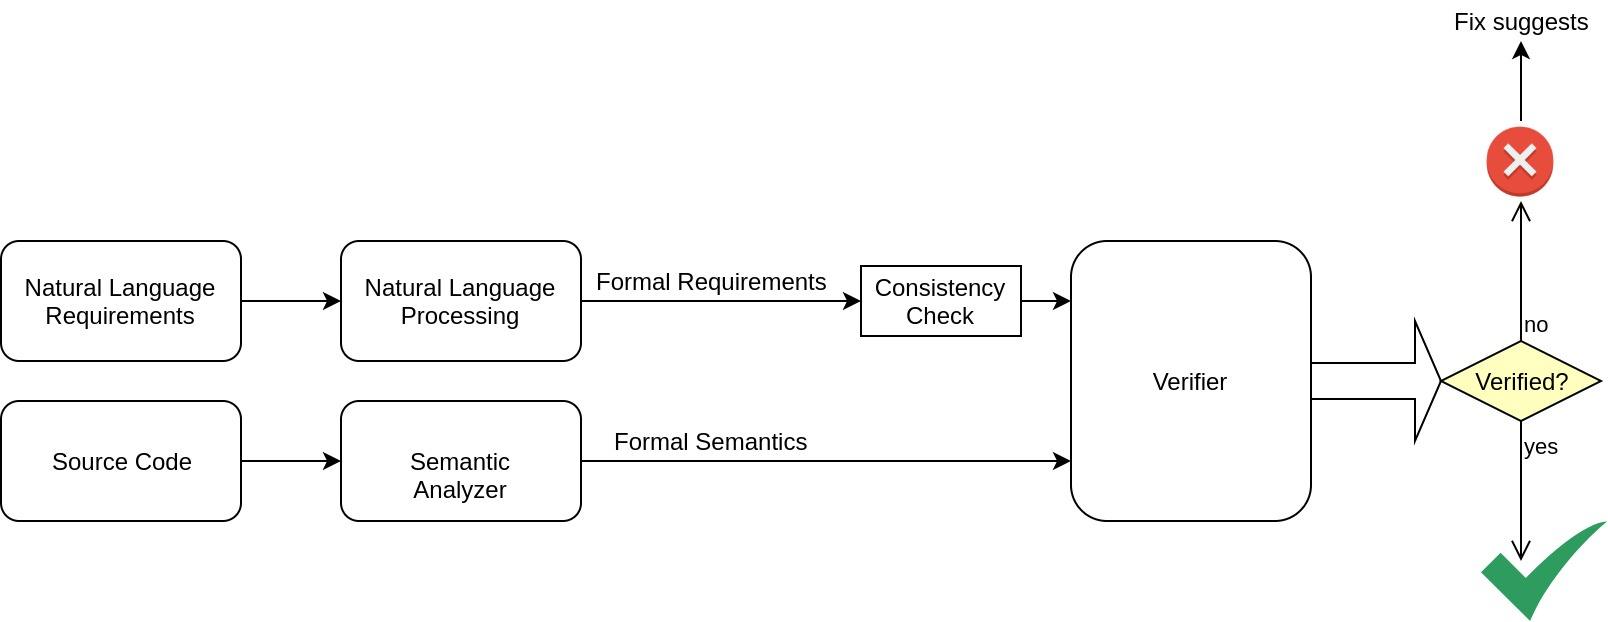
\includegraphics[width=1\linewidth]{../Architecture}
		\caption[PorjArch]{Project Architecture}
		\label{fig:architecture}
	\end{figure}
	
\begin{multicols*}{2}	
	\gls{NLP} is used for formalizing the \gls{SRS}. Since, natural language is widely understood by stakeholders, it is used as a common way for representing requirements. Representing requirements in natural language suffers from potential problems like ambiguity, inconsistency and incompleteness.
	
	One of the highest challenge in software engineering is developing software based on unclear requirements. Researches and literature reviews for the last 20 years shows that this is a known problem and big problem \cite{Besrour}. From the very beginning of software engineering, engineers, researchers and scientist used formal and semi-formal methods as a solution of this problem. Yet, initial requirements is written in natural language and there is no escape to avoid it, even by using formal and semi-formal methods \cite{Kamsties}. Moreover, in industrial projects stakeholders usually come from different areas and they may not know formal methods.
	
	Due to unclear requirements the software project development may lead to higher costs and effort, or even a failure in cases where requirements were not understood.
	Common problem, when two software developers interpret requirements differently, based on their point of view. Ferrari et al. (2014) asserted that subjective interpretation leads to software design which is different from the one what was expected in the requirements \cite{Ferrari}.
	
	In the last half century, \gls{SRS} processing and analysis has been one of the focus researching area in software engineering. Due to unclearness of natural language, computer automation of analyzing \gls{SRS} always was a huge challenge. Therefore, the analysis of \gls{SRS} is made manually, what requires time, high costs and effort. But most importantly, as it was mentioned above, the manual analysis of \gls{SRS} leads to imprecise and mistaken results \cite{Wang}. With higher number of requirement (hundreds \gls{SRS} documents containing thousands requirements) this problem will be even more critical and hardly avoidable. Hence, verifying thousands requirements manually by humans will lead to extremely high costs \cite{Fanmuy}.
	
	The importance of finding a way to automate \gls{SRS} processing is unarguably important, roughly, because the main source of problems in requirement engineering is its gross dependence on humans \cite{Ahmed}. As a possible solution to resolve unclearness and provide valuable and clear information to software developers is using \gls{NLP}.
	
	Ryan (1993) questioned that: ”It is highly questionable that the resulting system from \gls{NLP} would be of great use in requirements engineering” \cite{Ryan}.
	
	Nazir et al. (2017) worked on a systematic literature review on \gls{NLP} applications for software requirement engineering and he consummated that: “Manual operations are still required on initial plain text of software requirements before applying the desired \gls{NLP} techniques” \cite{Nazir}.
	
	Besides the \gls{NLP}, our work can create and analyze the formal semantics of the source code.  A formal semantics should serve as a solid foundation for any programming language development, so it must be correct and complete (to be trusted and useful), executable (to yield a reference implementation), and appropriate for program reasoning and verification.
	
	Several efforts to give C a formal semantics have been made, most notably by Charles McEwen Ellison (III.). His executable formal semantics of the C language successfully passes  99.2\% of 776 test programs \cite{Ellison:2012:EFS:2103621.2103719}. Having to define two or more different semantics for a real-life language, together with proofs of equivalence, is a huge burden in itself, not to mention that these all need to be maintained as the language evolves.
	
	Currently code validation falls into two categories: testing and formal verification. Formal verification mainly includes two methods: theorem proving and model checking.
	
	Theorem Proving requires considerable expertise to guide and assist the verification process, and can not generate counter-examples that are useful for debugging when the verification fails.
	
	Model Checking \cite{Clarke:2000:MC:332656} is an automatic formal verification technique for a finite state system, where all the states of the system are exhaustively enumerated and the correctness condition checked at each state. Moreover, model checking yields extremely useful counter examples if it fails. It has proven effective in detecting errors in hardware designs.
	
	Software model checking could produce major enhancements in software reliability and robustness. However, the state space of software programs is typically so huge that they cannot be directly model checked with conventional model checking methods. Fortunately, applying mathematically abstraction methods might extract a reduced model from a program which makes model checking feasible.
	
	Our goal is to tackle multiple problems listed above. Design and train an \gls{NLP} for reliably analyzing the requirements and to verify the semantics of the C source code against the given requirements.
	
\end{multicols*}



\section{Methods}
	\begin{multicols*}{2}
		[\subsection{\gls{SRS} analysis}
		\gls{SDLC} starts with eliciting the \gls{SRS}, noted by the stakeholders. As stakeholders use their own language to state their requirements, it is observed to be very often ambiguous and confusing to analyze and subsequently design the desired solution. On one side we only focus on \gls{SRS} requirement document which follows the IEEE-STD-830 standard in a textual form. In the other side \gls{NLP} concepts are found to be helpful for the analysis. \gls{NLP} system processes the data written in natural language in an intelligent manner and generates an information which is comparatively easier to analyze.\cite{Tripathy}]
		Using \gls{NLP} can help in:
		\begin{itemize}
			\item the syntax of natural language
			\item the lexical context of the words
			\item the semantic components which construct the literal meaning of a sentence
			\item the pragmatic components which construct non-literal meaning of a sentence
			\item the parser generating the phrase tree structure of a sentence.
		\end{itemize}
		\gls{POST} is a semantic analysis approach and deals with assigning one or more \gls{POS} to a given word. The different types of \gls{POS} are,
		\begin{itemize}
			\item Noun (names): a word or lexical item denoting any abstract (abstract noun: e.g. home) or concrete entity (concrete noun: e.g. house); a person (police officer, Michael), place (coastline, London), thing (necktie, television), idea (happiness), or quality (bravery). Nouns can also be classified as count nouns or non-count nouns; some can belong to either category. The most common part of speech; they are called naming words.
			\item Pronoun (replace or again placed): a substitute for a noun or noun phrase (them, he). Pronouns make sentences shorter and clearer since they replace nouns.
			\item Adjective (describes, limits): a modifier of a noun or pronoun (big, brave). Adjectives make the meaning of another word (noun) more precise.
			\item Verb (states action or being): a word denoting an action (walk), occurrence (happen), or state of being (be). Without a verb a group of words cannot be a clause or sentence.
			\item Adverb (describes, limits): a modifier of an adjective, verb, or another adverb (very, quite). Adverbs make language more precise.
			\item Preposition (relates): a word that relates words to each other in a phrase or sentence and aids in syntactic context (in, of). Prepositions show the relationship between a noun or a pronoun with another word in the sentence.
			\item Conjunction (connects): a syntactic connector; links words, phrases, or clauses (and, but). Conjunctions connect words or group of words.
			\item Interjection (expresses feelings and emotions): an emotional greeting or exclamation (Huzzah, Alas). Interjections express strong feelings and emotions.
			\item Article (describes, limits): a grammatical marker of definiteness (the) or indefiniteness (a, an). The article is not always listed among the parts of speech. It is considered by some grammarians to be a type of adjective or sometimes the term 'determiner' (a broader class) is used.
		\end{itemize}
		Identification of all these \gls{POS} makes the task of \gls{NLP} simpler.
		
		Following Fillmore’s idea of defining a universal set of cases and Nan Niu’s variation structure, Wang et al. introduce a set of extended dimensions for conceptualizing the functional variability structure\cite{5381217}. An \gls{EFRF} is composed by 10 different semantic cases. Thus, the following variation dimensions for an \gls{EFRF} are considered.
		\begin{itemize}
			\item Agentive defines the agent whose activities will occur in \gls{EFRF}’s affairs. For example, $\{\mbox{student}\}_{Agentive}$
			“do homework”.
			\item Action defines the main action of the activity. For
			example, “TA” $\{\mbox{mark}\}_{Action}$.
			\item Objective defines the object affected by the activity.
			For example, “mark” $\{\mbox{homework}\}_{Objective}$.
			\item Agentmod defines the feature of agent. For example,
			{Senior}Agentmod $\{\mbox{student}\}_{Agentive}$.
			\item Objmod defines the feature of object. For example,
			$\{\mbox{c++}\}_{Objmod} \{\mbox{homework}\}_{Objective}$.
			 \item Locational defines the location where the \gls{EFRF} affairs occur. For example, “do homework” $\{\mbox{at home}\}_{Locational}$.
			 \item Temporal defines the duration or frequency of the
			 \gls{EFRF}’s activity. For example, “mark homework” $\{\mbox{every Sunday}\}_{Temporal}$.
			 \item  Manner defines the way or tool by which the
			 \gls{EFRF}’s activity is performed. Some examples are,
			 “access Internet” via $\{\mbox{Ethernet, Wireless}\}_{Manner}$,
			 “mark assignment” through $\{\mbox{Internet}\}_{Manner}$.
			 \item Goal defines the goal of the \gls{EFRF}’s activity. For example, “do homework carefully” $\{\mbox{in order to get an A}\}_{Goal}$.
			 \item Constraint defines the requirement and constraint
			 that make the activity occur. For example, “do
			 homework on-line” if $\{\mbox{access Internet}\}_{Constraint}$.
		\end{itemize}
		This extended set reflects most grammatical features
		that are associated with functional requirements description;
		hence it can serve as a framework of categories that helps
		analysts understand the variation points, i.e. what can vary,
		of the \gls{EFRF}. The systematical and clear definition of these
		variable points can help the effectiveness of software product line's functional variability modeling. 

		\begin{minipage}{0.9\linewidth}
			\centering
			\begin{figure}[H]
				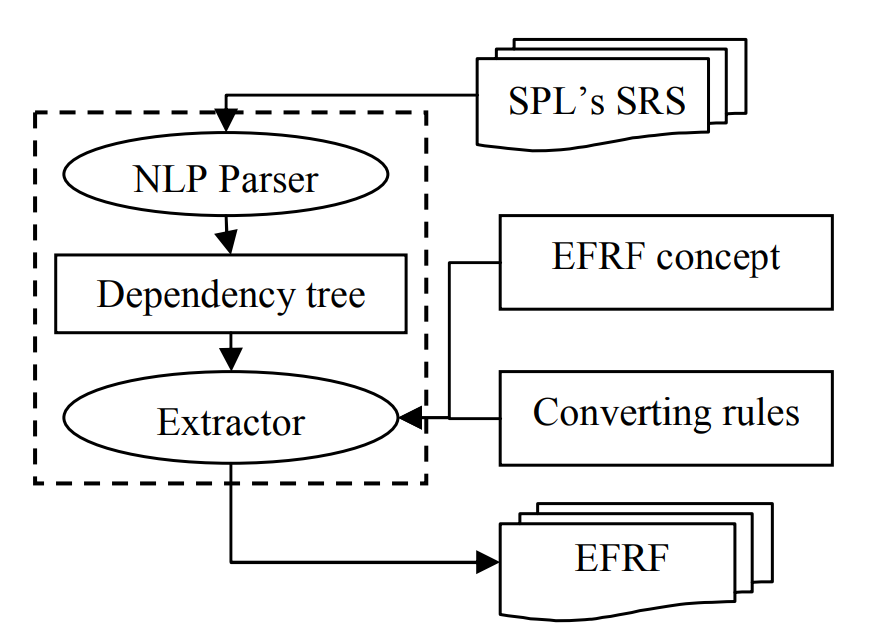
\includegraphics[width=\linewidth]{Architecture}
				\caption{Architecture}
				\label{fig:cc}
			\end{figure}
		\end{minipage}
		
		First the NLP Parser is the Stanford Parser \cite{stanfordParser} as the NLP parser. It can generate dependency trees to express the
		grammatical relations in sentences. The grammatical relations are arranged in a hierarchy, rooted with the most generic relation named “dependent”. Altogether, the hierarchy
		contains 48 grammatical relations. The whole hierarchy of
		the grammatical relations is given in \cite{Marneffe}.
		The second step is the Extractor, where the grammatical relations are converted into \gls{EFRF}s by converting rules which are introduce by \cite{5381217}. In this step, \gls{EFRF}s are merged which express the
		same functional requirements. If two \gls{EFRF}s describe the same
		activity, then they will be merged by combining their cases. 
		
	\end{multicols*}


\begin{minipage}{\linewidth}
	\begin{multicols*}{2}
		[
		\vspace{6 mm}
		\subsection{Semantic Analyzer}
		Despite C provides constructs that map to machine instructions, it also provides enough abstraction above \gls{asm} for developers to finish their work independently of platform  on which their C program runs.]
		Despite the abstraction mentioned above, C is known for the deftness in which it allows to developers to write programs with bugs. Despite there is no runtime error detection and just a little static analysis, in C the developers trust entirely. The C language is low-level enough despite its abstraction, so developers take advantage of supposition about the root architecture.  
		Back in time, the C standard was written in two of the design principles: the ability to develop a non-portable code and the trust in the programmer\cite{AmericanNationalStandardsInstitute:1990:RAC:533966}. Such principles also work together to create complex, platform-dependent bugs. The possible subtlety of C bugs makes them an ideal formalization candidate, as subtle bugs can often be found only by more thorough means.
		
		In this article, a formal semantics of \gls{MISRA} C is presented that is to be used to find bugs. "Formal semantics for realistic programming languages are large and complicated. This raises the question of validating these semantics: how can we make sure that they correctly capture the expected behaviors?" questions Blazy-Leroy in his "Mechanized semantics for the Clight subset of the C language" \cite{Blazy}. He writes how a subset of the C language can be formalized. Many uses of C in embedded or critical applications mandate strict coding guidelines restricting programmers to a “safer” subset of C \cite{HATTON2004465}. A well-known example is \gls{MISRA} C \cite{MISRA2004}. \gls{MISRA} C and Clight \cite{Blazy} share some restrictions (such as structured \textit{switch} statements with \textit{default} cases at the end), but otherwise differ significantly. For instance, \gls{MISRA} C prohibits recursive functions, but permits all uses of \textit{goto}. More generally, the restrictions of \gls{MISRA} C and related guidelines are driven by software engineering considerations and the desire for tool-assisted checking, while the restrictions of Clight stem from the desire to keep its formal semantics manageable.
	\end{multicols*}
\end{minipage}

\begin{minipage}{\linewidth}
	\begin{multicols*}{2}
		[
		\vspace{6 mm}
		\subsection{Consistency Check}
		Even though diverse techniques for
		requirements analysis and model derivation have been developed, problems still remain in this process, mainly related with the ambiguity, incompleteness and inconsistency of the documented requirements. Documenting high-quality software requirements that efficiently support the follow-up software analysis and design remains a classical challenge to the requirements engineering research community. ]
		Temp.
	\end{multicols*}
\end{minipage}



\section{Results}
\begin{minipage}{\linewidth}
	\begin{multicols*}{2}
		In this paper, we contributed an approach to extract functional requirements from free text documents for supporting domain analysis. We proposed an extended variability model to help the detailed and integrated expression of product line functional requirements. And then we automatically convert dependency relations of words in a sentence into cases to support the modeling of the variability of product line functional requirements. These pre-processed requirements could be fed to a recurrent neural network which could generate the semantic meaning og the natural language functional requirements. The performance of our \gls{RNN} can be seen in the following table.
	\end{multicols*}
		\begin{tabular}{|c|c|c|c|c|}\hline
			Metrics& LSTM Metics 30 lags &\vtop{\hbox{\strut LSTM Metrics}\hbox{\strut Optimal Time Lags}} &\vtop{\hbox{\strut Extra Tree}\hbox{\strut Model Metrics}} &Error Reduction (\%)\\\hline
			RMSE & 353.38 & 341.40 & 428.1 &20.3\\
			CV(RMSE)&0.643& 0.622& 0.78& 20.3\\
			MAE&263.14&249.53&292.49&14.9\\\hline
		\end{tabular}
	\begin{multicols*}{2}
		Another result is that we were able to define the full formal semantics of \gls{MISRA} C. We covered all cases and rules defined by \gls{MISRA} C. From this result we were able to analyze the formal semantics of various automotive C source codes. During our analysis we were able to spot multiple ambiguities and design faults. The semantic analysis itself can help improve the code quality and help avoid misunderstandings during the development procedure.
		
		At the end the semantics of the requirements and the semantics of the source code were compared against each other. The verifier is rigorously proven to be correct. It can check whether the given source is fulfilling the given functional requirements. If the verifier finds the source code incorrect than in some cases it can suggest fixes. The fixes are proved to be correct and we defined goodness measures for ranking these plausible fixes.
		
		All together we were able to build a development environment which rigorously supports the software development from the beginning to the end. All steps are mathematically proven to be correct and our result is a state of the art solution for a real life problem. During the process we overcome many obstacles and improved many algorithms and methodologies.
	\end{multicols*}
\end{minipage}


\section{Discussion}

\newpage
\bibliography{mybib}{}
\bibliographystyle{plain}

\newpage
\printglossary[type=\acronymtype]
\newpage
\printglossary[type=main]


\end{document}
